\chapter{Technical data information}
\label{chapter:Annexes}

\subsection{Database schema}
\label{chapter:Annex_schema}

This section provides an overview of all the tables that compose the data once the cleaning process is finished.

The first listing of tables corresponds to the information stored for each individual. The tables are divided by topics for better understanding, but mathematically, they should all be joined together by ID to create a large table for each of the FF time points (FF1, FF2, etc...).

\begin{sloppypar}
\begin{itemize}
    \item {Basic} (\textbf{ID}, Attendance Date FF1, Attendance Date FF12, Medication Date FF1, Questionary Date FF1, Sex, Age, General Health, Age FF12)

    \item {Network Technical} (\textbf{ID}, Signature FF1, Comment, Signature FF12, Comment FF12)
    
    \item {Antropometric FF1} (\textbf{ID}, Waist, Hip, Height, Weight, BMI, HR, SYSBP, DIABP, BMI Categorical)
    
    \item {Antropometric FF2} (\textbf{ID}, Waist, Hip, Height, Weight, BMI, HR, SYSBP, DIABP, BMI Categorical)

    \item {Aureus} (\textbf{ID}, S1 AttendanceDate, S1 R2 AttendanceDate, S2 AttendanceDate, S1 CultureDate, S2 CultureDate, S1 BacterialNasalGrowth, S1 BacterialThroatGrowth, S2 BacterialNasalGrowth, S2 BacterialThroatGrowth, S1 SA Direct NasalGrowth, S1 SA Direct ThroatGrowth, S1 SA Direct NasalPopulation, S1 SA Direct ThroatPopulation, S2 SA Direct NasalGrowth, S2 SA Direct ThroatGrowth, S2 SA Direct NasalPopulation, S2 SA Direct ThroatPopulation, S1 SA Enrich NasalGrowth, S1 SA Enrich ThroatGrowth, S1 SA Enrich NasalPopulation, S1 SA Enrich ThroatPopulation, S2 SA Enrich NasalGrowth, S2 SA Enrich ThroatGrowth, S2 SA Enrich NasalPopulation, S2 SA Enrich ThroatPopulation, S1 Direct CoagulaseNasal, S1 Direct CoagulaseThroat, S1 Enrich CoagulaseNasal, S1 Enrich CoagulaseThroat, S2 Direct CoagulaseNasal, S2 Direct CoagulaseThroat, S2 Enrich CoagulaseNasal, S2 Enrich CoagulaseThroat, SPANasal1, SPANasal2, SPAThroat1, SPAThroat2, SPAThroatClonning, SPAThroatCount, S1 D NasalColonize, S1 D ThroatColonize, S1 D Colonize, S1 E NasalColonize, S1 E ThroatColonize, S1 E Colonize, S2 D NasalColonize, S2 D ThroatColonize, S2 D Colonize, S2 E NasalColonize, S2 E ThroatColonize, S2 E Colonize, D NasalCarrier, D ThroatCarrier, D Carrier, E NasalCarrier, E ThroatCarrier, E Carrier, P Nasal, P Throat, P Carrier)

    \item {Swabbing} (\textbf{ID}, S1 NasalOK, S1 ThroatOK, S1 LabComments Enrich, S1 LabComments Staph, S1 Performed, S1 Event, S1 Medical Event, S1 Medical Event Comment, S1 Technical Event, S1 Technical Event Comment, S1 Abort Event, S1 Abort Event Comment, S1 Other Event, S1 Other Event Comment, S2 Performed, S2 Event, S2 Medical Event, S2 Medical Event Comment, S2 Technical Event, S2 Technical Event Comment, S2 Abort Event, S2 Abort Event Comment, S2 Other Event, S2 Other Event Comment, S1 Repeated Performed, S1 Nose Repeated, S1 Throat Repeated, S1 Repeated Event, S1 Repeated Medical Event, S1 Repeated Medical Event Comment, S1 Repeated Technical Event, S1 Repeated Technical Event Comment, S1 Repeated Abort Event, S1 Repeated Abort Event Comment, S1 Repeated Other Event, S1 Repeated Other Event Comment, S1 Nasal FreezeDate, S1 Throat FreezeDate, S1 FreezerNasalID, S1 FreezerThroatID, S2 FreezerNasalID, S2 FreezerThroatID)

    \item {High School} (\textbf{ID}, HighSchool, Class, Programme, MainPrograme)
    
    \item {Blood} (\textbf{ID}, Blood Analysis Date, Plasma Analysis Date, Time Since Eating, Mean Corposcular Hemoglobin pg, Mean Corposcular Hemoglobin Concentration g dL, Mean Corposcular Hemoglobin Volume fl, Fe µmol L, Ferritinin ug L, Transferrin g L, Total cholesterol mmol L, Triglycerides mmol L, LDL cholesterol mmol L, HDL cholesterol mmol L, Calcium mmol L, High sensitive CRP, Apolipoprotein A1 g L, Apolipoprotein B g L, Estradiol E2 nmol L, Progesterone nmol L, Testosterone nmol L, DHEA SO4 µmol L, SHBG nmol L, LH IU L, FSH IU L, Glucose Non fasting mmol L, HBA1C ..., Haemoglobin g dL, Albumin g L, X25 OH D nmol L, Retinol µmol L, PTH pmol L, FA C12 0 mcg ml, FA C14 0 mcg ml, FA C15 0 mcg ml, FA C16 0 mcg ml, FA C16 1 n 7 mcg ml, FA C18 0 mcg ml, FA C18 1 t6 11 mcg ml, FA C18 1 c 9 mcg ml, FA C18 1 c 11 mcg ml, FA C18 2 n 6 mcg ml, FA C20 0 mcg ml, FA C18 3 n 6 mcg ml, FA C18 3 n 3 mcg ml, FA C20 1 n 9 mcg ml, FA C20 2 n 6 mcg ml, FA C22 0 mcg ml, FA C20 3 n 6 mcg ml, FA C20 4 n 6 mcg ml, FA C23 0 mcg ml, FA C20 5 n 3 mcg ml, FA C24 0 mcg ml, FA C24 1 mcg ml, FA C22 5 n 3 mcg ml, FA C22 6 n 3 mcg ml, FA C12 0 weight, FA C14 0 weight, FA C15 0 weight, FA C16 0 weight, FA C16 1 n 7 weight, FA C18 0 weight, FA C18 1 t6 11 weight, FA C18 1 c 9 weight, FA C18 1 c 11 weight, FA C18 2 n 6 weight, FA C20 0 weight, FA C18 3 n 6 weight, FA C18 3 n 3 weight, FA C20 1 n 9 weight, FA C20 2 n 6 weight, FA C22 0 weight, FA C20 3 n 6 weight, FA C20 4 n 6 weight, FA C23 0 weight, FA C20 5 n 3 weight, FA C24 0 weight, FA C24 1 weight, FA C22 5 n 3 weight, FA C22 6 n 3 weight)
    
    \item {Blood Technical} (\textbf{ID}, Blood Test Performed, Blood Event, Blood Medical Event, Blood Medical Comment, Blood Technical Event, Blood Technical Comment, Blood Aborted, Blood Aborted Comment, Blood Other, Blood Other Comment, Blood S25OH Event, Blood S25OH Event Comment, Blood Retinol Event, Blood Retinol Event Comment)

    \item {Sociology} (\textbf{ID}, Live With Mother, Live With Father, Live With Stepfather, Live With Stepmother, Live With Foster Parents, Live With Adoptive Parents, Live With Grandparents, Live With Friends, Live With Nobody, Live With Institution, Live With Other, When Left Home, Mother Work Time, Mother Studying, Mother Domestic, Mother Disable, Father Work Time, Father Studying, Father Domestic, Father Disable, Mother Education, Father Education, Ethnicity, Live With Siblings)
    
    \item {Frienship Table} (\textbf{ID}, Created, Overview, Yesterday SMS, Overall Connections, Overall Popularity, Overall Following, Overall Reciprocity, Physical Connections, Physical Popularity, Physical Following, Physical Reciprocity, School Connections, School Popularity, School Following, School Reciprocity, Sports Connections, Sports Popularity, Sports Following, Sports Reciprocity, Home Connections, Home Popularity, Home Following, Home Reciprocity, Other Connections, Other Popularity, Other Following, Other Reciprocity, Overall Connections FF12, Overall Popularity FF12, Overall Following FF12, Overall Reciprocity FF12, Physical Connections FF12, Physical Popularity FF12, Physical Following FF12, Physical Reciprocity FF12, School Connections FF12, School Popularity FF12, School Following FF12, School Reciprocity FF12, Sports Connections FF12, Sports Popularity FF12, Sports Following FF12, Sports Reciprocity FF12, Home Connections FF12, Home Popularity FF12, Home Following FF12, Home Reciprocity FF12, Other Connections FF12, Other Popularity FF12, Other Following FF12, Other Reciprocity FF12)
    
    \item {Puberty Men Table} (\textbf{ID}, Change Height, Change Voice, Facial Hair, Men Body Hair, Men Pubic Hair, Men Pubic Age)
    
    \item {Puberty Women Table} (\textbf{ID}, Menarche, Menarche Age, Women Pubic Hair, Breasts)

    \item {Menstruation} (\textbf{ID}, Date, Menstruation Start, Menstruation Regular, Menstruation Cycle, Menstruation Date, Cycle Advance)
    
    \item {Drugs Table} (\textbf{ID}, Smoke, Smoke Per Week, Smoke Per Day, Snuff, Snuff Per Week, Snuff Per Day, Alcohol, Alcohol Units, Alcohol 6 Units)

    \item {Sports} (\textbf{ID}, Sports Leisure, Sports Outside School, Sports Frequency, Sport Hours, Sports Intensity, Summer Transport, Summer Time, Winter Transport, Winter Time, Screen Time)
    
    \item {Hygiene} (\textbf{ID}, Shower Bath Frequency, Handwash Frequency, Body Lotion Frequency, Skin Sunbathing, Holiday Sunbathing, Solarium Last 4 Weeks) 
    
    \item {Biomarkers} (\textbf{ID}, BatchNumber, Flagged, Adenosine Deaminase LOD, Artemin LOD, Axin 1 LOD, Brain derived neurotrophic factor LOD, Beta nerve growth factor LOD, Caspase 8 LOD, Eotaxin LOD, CC motif chemokine 19 LOD, CC motif chemokine 20 LOD, CC motif chemokine 23 LOD, CC motif chemokine 25 LOD, CC motif chemokine 28 LOD, CC motif chemokine 3 LOD, CC motif chemokine 4 LOD, Natural killer cell receptor 2B4 LOD, CD40L receptor LOD, T cell surface glycoprotein CD5 LOD, T cell surface glycoprotein CD6 isoform LOD, CUB domain containing protein 1 LOD, Macrophage colony stimulating factor 1 LOD, Cystatin D LOD, Fractalkine LOD, CXC motif chemokine 1 LOD, CXC motif chemokine 10 LOD, CXC motif chemokine 11 LOD, CXC motif chemokine 5 LOD, CXC motif chemokine 6 LOD, CXC motif chemokine 9 LOD, Delta and Notch like epidermal growth factor related receptor LOD, Eukaryotic translation initiation factor 4E binding protein 1 LOD, Protein S100 A12 LOD, Fibroblast growth factor 19 LOD, Fibroblast growth factor 21 LOD, Fibroblast growth factor 23 LOD, Fibroblast growth factor 5 LOD, Fms related tyrosine kinase 3 ligand LOD, Glial cell line derived neurotrophic factor LOD, Hepatocyte growth factor LOD, Interferon gamma LOD, Interleukin 10 LOD, Interleukin 10 receptor subunit alpha LOD, Interleukin 10 receptor subunit beta LOD, Interleukin 12 subunit beta LOD, Interleukin 13 LOD, Interleukin 15 receptor subunit alpha LOD, Interleukin 17 A LOD, Interleukin 17 C LOD, Interleukin 18 LOD, Interleukin 18 receptor 1 LOD, Interleukin 1 alpha LOD, Interleukin 2 LOD, Interleukin 20 LOD, Interleukin 20 receptor subunit alpha LOD, Interleukin 22 receptor subunit alpha 1 LOD, Interleukin 24 LOD, Interleukin 2 receptor subunit beta LOD, Interleukin 33 LOD, Interleukin 4 LOD, Interleukin 5 LOD, Interleukin 6 LOD, Interleukin 7 LOD, Interleukin 8 LOD, Leukemia inhibitory factor LOD, Leukemia inhibitory factor receptor LOD, Monocyte chemotactic protein 1 LOD, Monocyte chemotactic protein 2 LOD, Monocyte chemotactic protein 3 LOD, Monocyte chemotactic protein 4 LOD, Matrix metalloproteinase 1 LOD, Matrix metalloproteinase 10 LOD, Neurturin LOD, Neurotrophin 3 LOD, Osteoprotegerin LOD, Oncostatin M LOD, Programmed cell death 1 ligand 1 LOD, Stemcell factor LOD, SIR2 like protein 2 LOD, Signaling lymphocytic activation molecule LOD, Sulfotransferase 1A1 LOD, STAM binding protein LOD, Transforming growth factor alpha LOD, Latency associated peptide transforming growth factor beta 1 LOD, Tumor necrosis factor LOD, TNF beta LOD, Tumor necrosis factor receptor superfamily member 9 LOD, Tumor necrosis factor ligand superfamily member 14 LOD, TNF related apoptosis inducing ligand LOD, TNF related activation induced cytokine LOD, Thymic stromal lymphopoietin LOD, Tumor necrosis factor LOD, Urokinase type plasminogen activator LOD, Vascular endothelial growth factor A LOD, Adenosine Deaminase NLD, Artemin NLD, Axin 1 NLD, Brain derived neurotrophic factor NLD, Beta nerve growth factor NLD, Caspase 8 NLD, Eotaxin NLD, CC motif chemokine 19 NLD, CC motif chemokine 20 NLD, CC motif chemokine 23 NLD, CC motif chemokine 25 NLD, CC motif chemokine 28 NLD, CC motif chemokine 3 NLD, CC motif chemokine 4 NLD, Natural killer cell receptor 2B4 NLD, CD40L receptor NLD, T cell surface glycoprotein CD5 NLD, T cell surface glycoprotein CD6 isoform NLD, CUB domain containing protein 1 NLD, Macrophage colony stimulating factor 1 NLD, Cystatin D NLD, Fractalkine NLD, CXC motif chemokine 1 NLD, CXC motif chemokine 10 NLD, CXC motif chemokine 11 NLD, CXC motif chemokine 5 NLD, CXC motif chemokine 6 NLD, CXC motif chemokine 9 NLD, Delta and Notch like epidermal growth factor related receptor NLD, Eukaryotic translation initiation factor 4E binding protein 1 NLD, Protein S100 A12 NLD, Fibroblast growth factor 19 NLD, Fibroblast growth factor 21 NLD, Fibroblast growth factor 23 NLD, Fibroblast growth factor 5 NLD, Fms related tyrosine kinase 3 ligand NLD, Glial cell line derived neurotrophic factor NLD, Hepatocyte growth factor NLD, Interferon gamma NLD, Interleukin 10 NLD, Interleukin 10 receptor subunit alpha NLD, Interleukin 10 receptor subunit beta NLD, Interleukin 12 subunit beta NLD, Interleukin 13 NLD, Interleukin 15 receptor subunit alpha NLD, Interleukin 17 A NLD, Interleukin 17 C NLD, Interleukin 18 NLD, Interleukin 18 receptor 1 NLD, Interleukin 1 alpha NLD, Interleukin 2 NLD, Interleukin 20 NLD, Interleukin 20 receptor subunit alpha NLD, Interleukin 22 receptor subunit alpha 1 NLD, Interleukin 24 NLD, Interleukin 2 receptor subunit beta NLD, Interleukin 33 NLD, Interleukin 4 NLD, Interleukin 5 NLD, Interleukin 6 NLD, Interleukin 7 NLD, Interleukin 8 NLD, Leukemia inhibitory factor NLD, Leukemia inhibitory factor receptor NLD, Monocyte chemotactic protein 1 NLD, Monocyte chemotactic protein 2 NLD, Monocyte chemotactic protein 3 NLD, Monocyte chemotactic protein 4 NLD, Matrix metalloproteinase 1 NLD, Matrix metalloproteinase 10 NLD, Neurturin NLD, Neurotrophin 3 NLD, Osteoprotegerin NLD, Oncostatin M NLD, Programmed cell death 1 ligand 1 NLD, Stemcell factor NLD, SIR2 like protein 2 NLD, Signaling lymphocytic activation molecule NLD, Sulfotransferase 1A1 NLD, STAM binding protein NLD, Transforming growth factor alpha NLD, Latency associated peptide transforming growth factor beta 1 NLD, Tumor necrosis factor NLD, TNF beta NLD, Tumor necrosis factor receptor superfamily member 9 NLD, Tumor necrosis factor ligand superfamily member 14 NLD, TNF related apoptosis inducing ligand NLD, TNF related activation induced cytokine NLD, Thymic stromal lymphopoietin NLD, Tumor necrosis factor NLD, Urokinase type plasminogen activator NLD, Vascular endothelial growth factor A NLD)
    
    \item {Diet} (\textbf{ID}, Breakfast Frequency, Fat Fish Frequency, Lean Fish Frequency, Seagull Eggs Frequency, Reindeer Frequency, Cheese Frequency, Chocolate Frequency, Fruits Frequency, Vegetables Frequency, Dairy Frequency, Fruit Juice Frequency, Sugar Juice Frequency, Sugar Drink Frequency, Sweetener Drink Frequency, Water Frequency, Fish Oil Frequency, Vitamins Frequency) 
    
    \item {Sleep} (\textbf{ID}, Hours Sleeping, Bed Time Hour Categorical, Bed Time Hour Float, Sleeping Pills)
    
\end{itemize}
\end{sloppypar}

The following tables describe the data that can be found in the relations described in figure \ref{fig:Database_relational_image}; this is, however, in melted form as described in the methodology.

\begin{itemize}

    \item {Diseases} (\textbf{ID}, Diagnostic, ICD10, Title, Age Diagnostic, Age Debut)     
    
    \item {Contraceptives} (\textbf{ID}, Brand, ATC, Type, Hormonal) 
    
    \item {Medicines} (\textbf{ID}, Type, Brand, ATC, Regularity, Content)        
\end{itemize}

Finally, for each of the six networks, we have a simplified version of the "Frienship" table described above. Here, we give an example of the physical network. The other five have the same structure but with just different names.

\begin{itemize}
    \item {Physical Edges} (\textbf{from}, \textbf{to}, value)     
\end{itemize}

\subsection{Data cleaning tables}

\subsubsection{Metadata information}

This section aims to inform about data shortcomings, so it can be replicated properly.

The original file with all the data description for all variables is called \detokenize{"20180601-Komplett Metadata FF1.xls"}, here we can find 1514 different variables across many different topics. But this file doesn't contain all the possible variable descriptions and what the numerical values mean when encoding categorical data.

Without the complete data specification, a good data logic system that retrieves the data properly can't be designed properly and this is a well-known source of errors, bugs, and patches. It also limited the analysis since the validation of values is not possible (i.e.: Is glucose above 300 biologically possible in our glucose variable?).

%can be designed from start while programming. Sometimes, the definitions in this document contradict what you find in the actual data, such as numbers in a column that don't appear in the specification. This means that instead of designing a robust data-cleaning script from scratch, it needs to be updated every time new information comes afloat, which in software development is a well-known source of errors, bugs, and patches.


\subsubsection{ \textit{S. Aureus} information}

\begin{table}[H]

	\tiny	

    \centering

    \label{table:SA_Original_Data_1}
    
	\renewcommand{\arraystretch}{1.5}

    \scalebox{0.85}{

    \begin{tabular}{| l | p{10cm} }
        \hline
        
        \rowcolor[HTML]{FFAAAA}
        \textbf{Name} & \textbf{Description} \\ 
        \hline 

        \rowcolor[HTML]{FFD1AA}        
		\multicolumn{2}{|l|}{Dates of attendance}   \\
		\hline      
        
        
        \multicolumn{1}{l|}{\detokenize{SWAB_DATE_FF1}}   & Attendance date for sample 1, for FF1. \\         
        \multicolumn{1}{l|}{\detokenize{SWAB_DATE_2_FF1}} & Attendance date for repetition of sample 1, for FF1. \\         
        \multicolumn{1}{l|}{\detokenize{SWAB_DATE_FF12}}  & Attendance date for sample 2, for FF1. \\                 
        
        
        \rowcolor[HTML]{FFD1AA}        
		\multicolumn{2}{|l|}{Dates of culture}   \\
		\hline              
                
        \multicolumn{1}{l|}{\detokenize{DATE_CULTURE_DAY0_FF1}}
        & Nasal and Throat sample 1 swabs for FF1, date of culturing in the laboratory. \\         
        
        
        \rowcolor[HTML]{FFD1AA}        
		\multicolumn{2}{|l|}{The experiment grew something in the agar plate}   \\
		\hline              
        
        
        \multicolumn{1}{l|}{\detokenize{CONTROL_NASAL_DAY2_FF1}}
        & Nasal swab, sample 1, FF1: Any growth of bacterial colonies on the control agar plate.  \\         
        \multicolumn{1}{l|}{\detokenize{CONTROL_THROAT_DAY2_FF1}}
        & Throat swab, sample 1, FF1: Any growth of bacterial colonies on the control agar plate. \\
        \multicolumn{1}{l|}{\detokenize{CONTROL_NASAL_DAY2_FF11}}
        & Nasal swab, sample 2, FF1: Any growth of bacterial colonies on the control agar plate.  \\         
        \multicolumn{1}{l|}{\detokenize{CONTROL_THROAT_DAY2_FF11}}
        & Throat swab, sample 2, FF1: Any growth of bacterial colonies on the control agar plate. \\

        \rowcolor[HTML]{FFD1AA}        
		\multicolumn{2}{|l|}{The experiment grew SA in the agar plate, Direct Culture}   \\
		\hline              

        
        \multicolumn{1}{l|}{\detokenize{STAPH_NASAL_DAY2_FF1}}
        & Nasal swab direct culture, sample 1, FF1: Any growth of bacterial colonies on Staphylococcus aureus selective agar plate. \\       
        \multicolumn{1}{l|}{\detokenize{STAPH_THROAT_DAY2_FF1}}
        & Throat swab direct culture, sample 1, FF1: Any growth of bacterial colonies on Staphylococcus aureus selective agar plate.\\         
        \multicolumn{1}{l|}{\detokenize{STAPH_GROWTH_NASAL_DAY2_FF1}}
        & Nasal swab direct culture, sample 1, FF1: Classification of growth of bacterial colonies on Staphylococcus aureus selective agar plate.  \\
        \multicolumn{1}{l|}{\detokenize{STAPH_GROWTH_THROAT_DAY2_FF1}}
        & Throat swab direct culture, sample 1, FF1: Classification of growth of bacterial colonies on Staphylococcus aureus selective agar plate\\         
        \multicolumn{1}{l|}{\detokenize{STAPH_NASAL_DAY2_FF11}}
        & Nasal swab direct culture, sample 2, FF1: Any growth of bacterial colonies on Staphylococcus aureus selective agar plate. \\       
        \multicolumn{1}{l|}{\detokenize{STAPH_THROAT_DAY2_FF11}}
        & Throat swab direct culture, sample 2, FF1: Any growth of bacterial colonies on Staphylococcus aureus selective agar plate.\\         
        \multicolumn{1}{l|}{\detokenize{STAPH_GROWTH_NASAL_DAY2_FF11}}
        & Nasal swab direct culture, sample 2, FF1: Classification of growth of bacterial colonies on Staphylococcus aureus selective agar plate.  \\
        \multicolumn{1}{l|}{\detokenize{STAPH_GROWTH_THROAT_DAY2_FF11}}
        & Throat swab direct culture, sample 2, FF1: Classification of growth of bacterial colonies on Staphylococcus aureus selective agar plate\\                 
        
        
        
        \rowcolor[HTML]{FFD1AA}        
		\multicolumn{2}{|l|}{The experiment grew SA in the agar plate, Enrichment Broth}   \\
		\hline              
        

        \multicolumn{1}{l|}{\detokenize{STAPH_NASAL_ENRICH_FF1}}
        & Nasal swab in enrichment broth, sample 1, FF1: Any growth on Staphylococcus aureus selective agar plate after enrichment\\         
        \multicolumn{1}{l|}{\detokenize{STAPH_THROAT_ENRICH_FF1}}
        & Throat swab in enrichment broth, sample 1, FF1: Any growth on Staphylococcus aureus selective agar plate after enrichment\\                
        \multicolumn{1}{l|}{\detokenize{STAPH_GROWTH_NASAL_ENRICH_FF1}}
        & Nasal swab in enrichment broth, sample 1, FF1: Classification of growth of bacterial colonies on Staphylococcus aureus selective agar plate after enrichment.\\
        \multicolumn{1}{l|}{\detokenize{STAPH_GROWTH_THROAT_ENRICH_FF1}}
        & Throat swab in enrichment broth, sample 1, FF1: Classification of growth of bacterial colonies on Staphylococcus aureus selective agar plate after enrichment\\
        \multicolumn{1}{l|}{\detokenize{STAPH_NASAL_ENRICH_FF11}}
        & Nasal swab in enrichment broth, sample 2, FF1: Any growth on Staphylococcus aureus selective agar plate after enrichment\\         
        \multicolumn{1}{l|}{\detokenize{STAPH_THROAT_ENRICH_FF11}}
        & Throat swab in enrichment broth, sample 2, FF1: Any growth on Staphylococcus aureus selective agar plate after enrichment\\                
        \multicolumn{1}{l|}{\detokenize{STAPH_GROWTH_NASAL_ENRICH_FF11}}
        & Nasal swab in enrichment broth, sample 2, FF1: Classification of growth of bacterial colonies on Staphylococcus aureus selective agar plate after enrichment.\\
        \multicolumn{1}{l|}{\detokenize{STAPH_GROWTH_THROAT_ENRICH_FF11}}
        & Throat swab in enrichment broth, sample 2, FF1: Classification of growth of bacterial colonies on Staphylococcus aureus selective agar plate after enrichment\\

        
        \rowcolor[HTML]{FFD1AA}        
		\multicolumn{2}{|l|}{Coagulase test to check for the presence of S. Aureus (positive) or S.Epidermitis or S.Saprophyticus (negative).}\\
		\hline                      
        
        \multicolumn{1}{l|}{\detokenize{STAPH_COAGULASE_NASAL_FF1}}
        & Nasal swab direct culture, sample 1, FF1: Coagulase test. \\         
        \multicolumn{1}{l|}{\detokenize{STAPH_COAGULASE_THROAT_FF1}}
        & Throat swab direct culture, sample 1, FF1: Coagulase test\\         
        \multicolumn{1}{l|}{\detokenize{STAPH_COAG_NASAL_ENRICH_FF1}}
        & Nasal swab in enrichment broth, sample 1, FF1: Coagulase test.\\         
        \multicolumn{1}{l|}{\detokenize{STAPH_COAG_THROAT_ENRICH_FF1}}
        & Throat swab in enrichment broth, sample 1, FF1: Coagulase test \\                 
        \multicolumn{1}{l|}{\detokenize{STAPH_COAGULASE_NASAL_FF11}}
        & Nasal swab direct culture, sample 2, FF1: Coagulase test. \\         
        \multicolumn{1}{l|}{\detokenize{STAPH_COAGULASE_THROAT_FF11}}
        & Throat swab direct culture, sample 2, FF1: Coagulase test\\         
        \multicolumn{1}{l|}{\detokenize{STAPH_COAG_NASAL_ENRICH_FF11}}
        & Nasal swab in enrichment broth, sample 2, FF1: Coagulase test.\\         
        \multicolumn{1}{l|}{\detokenize{STAPH_COAG_THROAT_ENRICH_FF11}}
        & Throat swab in enrichment broth, sample 2, FF1: Coagulase test \\                 



        \rowcolor[HTML]{FFD1AA}        
		\multicolumn{2}{|l|}{SPA-Typing variables.}\\
		\hline                      
        

        \multicolumn{1}{l|}{\detokenize{SPA_THROAT1_FF1}}& Throat swab: Spa-type of S. aureus isolate. \\         
        \multicolumn{1}{l|}{\detokenize{CCN_THROAT1_FF1}}& (Not described in the metadata). \\         
        \multicolumn{1}{l|}{\detokenize{CC_THROAT1_FF1}} & Throat swab: S. aureus clonal complex based on spa-type.\\         
        \multicolumn{1}{l|}{\detokenize{SPA_NASAL1_FF1}} & Nasal swab: Spa-type of S. aureus isolate.\\         
        \multicolumn{1}{l|}{\detokenize{SPA_NASAL2_FF1}} & Second nasal swab: Spa-type of S. aureus isolate.\\         
        \multicolumn{1}{l|}{\detokenize{SPA_THROAT2_FF1}}& (Not described in the metadata). \\      
            
    \end{tabular}%
    }
    \caption{Table with the original data for the S.Aureus variables.}
    
\end{table}


\subsubsection{S. Aureus mapping}

\begin{table}[H]

	\tiny

	\centering

    \label{table:Table_SA_Transform_Categories}
    
	\renewcommand{\arraystretch}{1.5}

    \begin{tabular}{l | l | l}
		\hline
        \rowcolor[HTML]{FF9999}		
		
        \textbf{Variable} & \textbf{Original} & \textbf{Transformed} \\ 		
        
        \hline 

            \multirow{4}{*}{S1$\_$BacterialNasalGrowth}
                                         & \multicolumn{1}{l}{1}     & \multicolumn{1}{l}{Yes}            \\\cline{2-3}
                                         & \multicolumn{1}{l}{0}     & \multicolumn{1}{l}{No}             \\\cline{2-3}
                                         & \multicolumn{1}{l}{9}     & \multicolumn{1}{l}{Non-applicable} \\\cline{2-3}
                                         & \multicolumn{1}{l}{NA}    & \multicolumn{1}{l}{Unknown}        \\\hline
                                    
            \multirow{4}{*}{S1$\_$SA$\_$Direct$\_$NasalGrowth} 
                                         & \multicolumn{1}{l}{1}     & \multicolumn{1}{l}{Yes}            \\\cline{2-3}
                                         & \multicolumn{1}{l}{0}     & \multicolumn{1}{l}{No}             \\\cline{2-3}
                                         & \multicolumn{1}{l}{9}     & \multicolumn{1}{l}{Non-applicable} \\\cline{2-3}
                                         & \multicolumn{1}{l}{NA}    & \multicolumn{1}{l}{Unknown}        \\\hline

            \multirow{5}{*}{S1$\_$SA$\_$Direct$\_$NasalPopulation} 
                                         & \multicolumn{1}{l}{0}  & \multicolumn{1}{l}{Light}          \\\cline{2-3}
                                         & \multicolumn{1}{l}{1}  & \multicolumn{1}{l}{Moderate}       \\\cline{2-3}
                                         & \multicolumn{1}{l}{2}  & \multicolumn{1}{l}{Rich}           \\\cline{2-3}
					                     & \multicolumn{1}{l}{NA} & \multicolumn{1}{l}{None}           \\\cline{2-3}
                                         & \multicolumn{1}{l}{9}  & \multicolumn{1}{l}{Non-applicable} \\\hline
                                         
            \multirow{4}{*}{S1$\_$SA$\_$Enrich$\_$NasalGrowth} 
                                         & \multicolumn{1}{l}{1}     & \multicolumn{1}{l}{Yes}            \\\cline{2-3}
                                         & \multicolumn{1}{l}{0}     & \multicolumn{1}{l}{No}             \\\cline{2-3}
                                         & \multicolumn{1}{l}{9}     & \multicolumn{1}{l}{Non-applicable} \\\cline{2-3}
                                         & \multicolumn{1}{l}{NA}    & \multicolumn{1}{l}{Unknown}        \\\hline

            \multirow{5}{*}{S1$\_$SA$\_$Enrich$\_$NasalPopulation} 
                                         & \multicolumn{1}{l}{0}  & \multicolumn{1}{l}{Light}          \\\cline{2-3}
                                         & \multicolumn{1}{l}{1}  & \multicolumn{1}{l}{Moderate}       \\\cline{2-3}
                                         & \multicolumn{1}{l}{2}  & \multicolumn{1}{l}{Rich}           \\\cline{2-3}
					                     & \multicolumn{1}{l}{NA} & \multicolumn{1}{l}{None}           \\\cline{2-3}
                                         & \multicolumn{1}{l}{9}  & \multicolumn{1}{l}{Non-applicable} \\\hline

            \multirow{4}{*}{S1$\_$Direct$\_$CoagulaseNasal} 
                                         & \multicolumn{1}{l}{1}     & \multicolumn{1}{l}{Positive}       \\\cline{2-3}
                                         & \multicolumn{1}{l}{0}     & \multicolumn{1}{l}{Negative}       \\\cline{2-3}
                                         & \multicolumn{1}{l}{9}     & \multicolumn{1}{l}{Non-applicable} \\\cline{2-3}
                                         & \multicolumn{1}{l}{Other} & \multicolumn{1}{l}{Unknown}        \\\hline

            \multirow{4}{*}{S1$\_$Enrich$\_$CoagulaseNasal} 
                                         & \multicolumn{1}{l}{1}     & \multicolumn{1}{l}{Positive}       \\\cline{2-3}
                                         & \multicolumn{1}{l}{0}     & \multicolumn{1}{l}{Negative}       \\\cline{2-3}
                                         & \multicolumn{1}{l}{9}     & \multicolumn{1}{l}{Non-applicable} \\\cline{2-3}
                                         & \multicolumn{1}{l}{Other} & \multicolumn{1}{l}{Unknown}        \\\hline

        \end{tabular}

    \caption{New values for the S.Aureus categories.}

\end{table}

\subsubsection{Swabbing}

\begin{table}[H]

	\tiny	

    \centering

    \label{table:Swabbing_Original_Data}
    
	\renewcommand{\arraystretch}{1.5}

    \scalebox{0.85}{

    \begin{tabular}{| l | p{10cm} }
        \hline
        
        \rowcolor[HTML]{FFAAAA}
        \textbf{Name} & \textbf{Description} \\ 
        \hline 

        \rowcolor[HTML]{FFD1AA}        
		\multicolumn{2}{|l|}{Information about trying to do the swabbing for the first time}   \\
		\hline      
        
        
        \multicolumn{1}{l|}{\detokenize{NASAL_SAMPLE_OK_FF1}}  & The swabbing in the nose was performed \\         
        \multicolumn{1}{l|}{\detokenize{THROAT_SAMPLE_OK_FF1}} & The swabbing in the throat was performed \\         

        
        \rowcolor[HTML]{FFD1AA}        
		\multicolumn{2}{|l|}{Lab comments}   \\
		\hline             

        \multicolumn{1}{l|}{\detokenize{LAB_COMMENTS_DAY0_FF1}} & Laboratory comments regarding the sample 1 \\         
        \multicolumn{1}{l|}{\detokenize{LAB_COMMENTS_DAY2_FF1}} & Laboratory comments regarding the sample 2 \\         		
		 
        \rowcolor[HTML]{FFD1AA}        
		\multicolumn{2}{|l|}{Enrich and Direct culture comments}   \\
		\hline    
		
        \multicolumn{1}{l|}{\detokenize{LAB_COMMENTS_ENRICH_FF1}} & Laboratory comments regarding the enrichment process. \\         
        \multicolumn{1}{l|}{\detokenize{COMMENTS_STAPH_FF1}}  & Laboratory comments regarding the direct culture. \\         				         		 
        \rowcolor[HTML]{FFD1AA}        
		\multicolumn{2}{|l|}{The swabbing was performed but something happened}   \\
		\hline            

        \rowcolor[HTML]{88CC88}        
		\multicolumn{2}{|l|}{For sample 1}   \\
		\hline            
        
        \multicolumn{1}{l|}{\detokenize{status_swab_ff1}}             & Swabbing was done \\         
        \multicolumn{1}{l|}{\detokenize{event_swab_ff1}}              & Something happened during the swabbing \\         		        
        
        \multicolumn{1}{l|}{\detokenize{event_swab_med_ff1}}          & Something medical related happened \\         
        \multicolumn{1}{l|}{\detokenize{event_swab_med_comment_ff1}}  & Comment about it\\         		                
        
        \multicolumn{1}{l|}{\detokenize{event_swab_tech_ff1}}         & Something technical related happened \\         
        \multicolumn{1}{l|}{\detokenize{event_swab_tech_comment_ff1}} & Comment about it\\         		                

        \multicolumn{1}{l|}{\detokenize{event_swab_abort_ff1}}         & Swabbing was aborted\\         
        \multicolumn{1}{l|}{\detokenize{event_swab_abort_comment_ff1}} & Comment about it\\         		                
        
        \multicolumn{1}{l|}{\detokenize{event_swab_other_ff1}}         & Something else happened\\         
        \multicolumn{1}{l|}{\detokenize{event_swab_other_comment_ff1}} & Comment about it\\         		                
        
        \rowcolor[HTML]{88CC88}        
		\multicolumn{2}{|l|}{For sample 2}   \\
		\hline            
        
        \multicolumn{1}{l|}{\detokenize{status_swab_ff12}}             & Swabbing was done \\         
        \multicolumn{1}{l|}{\detokenize{event_swab_ff12}}              & Something happened during the swabbing \\         		        
        
        \multicolumn{1}{l|}{\detokenize{event_swab_med_ff12}}          & Something medical related happened \\         
        \multicolumn{1}{l|}{\detokenize{event_swab_med_comment_ff12}}  & Comment about it\\         		                
        
        \multicolumn{1}{l|}{\detokenize{event_swab_tech_ff12}}         & Something technical related happened \\         
        \multicolumn{1}{l|}{\detokenize{event_swab_tech_comment_ff12}} & Comment about it\\         		                

        \multicolumn{1}{l|}{\detokenize{event_swab_abort_ff12}}         & Swabbing was aborted\\         
        \multicolumn{1}{l|}{\detokenize{event_swab_abort_comment_ff12}} & Comment about it\\         		                
        
        \multicolumn{1}{l|}{\detokenize{event_swab_other_ff12}}         & Something else happened\\         
        \multicolumn{1}{l|}{\detokenize{event_swab_other_comment_ff12}} & Comment about it\\         		        
        
        \rowcolor[HTML]{FFD1AA}        
		\multicolumn{2}{|l|}{The swabbing was repeated, and if so, something happened}   \\
		\hline            

        \rowcolor[HTML]{88CC88}        
		\multicolumn{2}{|l|}{For sample 1}   \\
		\hline                    

        \multicolumn{1}{l|}{\detokenize{status_swab_2_ff1}}           & Repetition of the swabbing was done \\         
        \multicolumn{1}{l|}{\detokenize{swab_nose_2_ff1}}             & Swabbing in the nose was repeated \\         		                
        \multicolumn{1}{l|}{\detokenize{swab_throat_2_ff1}}           & Swabbing in the throat was repeated \\         		                
        \multicolumn{1}{l|}{\detokenize{EVENT_SWAB_2_FF1}}            & Something happened during the repeated swabbing \\         		        
        
        \multicolumn{1}{l|}{\detokenize{event_swab_med_2_ff1}}          & Something medical happened \\         
        \multicolumn{1}{l|}{\detokenize{event_swab_med_comment_2_ff1}}  & Comment about it\\         		                
        
        \multicolumn{1}{l|}{\detokenize{event_swab_tech_2_ff1}}         & Something technical happened \\         
        \multicolumn{1}{l|}{\detokenize{event_swab_tech_comment_2_ff1}} & Comment about it\\         		                

        \multicolumn{1}{l|}{\detokenize{event_swab_abort_2_ff1}}         & Swabbing was aborted\\         
        \multicolumn{1}{l|}{\detokenize{event_swab_abort_comment_2_ff1}} & Comment about it\\         		                
        
        \multicolumn{1}{l|}{\detokenize{event_swab_other_2_ff1}}         & Something else happened\\         
        \multicolumn{1}{l|}{\detokenize{event_swab_other_comment_2_ff1}} & Comment about it\\          
        
        \rowcolor[HTML]{FFD1AA}        
		\multicolumn{2}{|l|}{Freezing the samples}   \\
		\hline                    
        
        \multicolumn{1}{l|}{\detokenize{DATE_FREEZE_STAPH_NASAL_FF1}}     & Date when freezing the nasal sample 1\\         
        \multicolumn{1}{l|}{\detokenize{DATE_FREEZE_STAPH_THROAT_FF1}}    & Date when freezing the throat sample 1\\         		                        
        \multicolumn{1}{l|}{\detokenize{freeze_number_staph_nasal_ff1}}   & Freezing nasal sample 1 ID\\         
        \multicolumn{1}{l|}{\detokenize{freeze_number_staph_throat_ff1}}  & Freezing throat sample 1 ID\\         
        
        \multicolumn{1}{l|}{\detokenize{freeze_number_staph_nasal_ff11}}  & Freezing nasal sample 2 ID\\         
        \multicolumn{1}{l|}{\detokenize{freeze_number_staph_throat_ff11}} & Freezing throat sample 2 ID\\         

    \end{tabular}%

    }

    \caption{Table with the original data about technical information regarding the swabbing.}
    
\end{table}


\subsubsection{School and education}

\begin{table}[H]

	\tiny	

    \centering

    \label{table:school_and_education_Original_Data}

	\renewcommand{\arraystretch}{1.5}

    \begin{tabular}{| l | p{10cm}  l }
    
        \hline
        \rowcolor[HTML]{FFAAAA}

        \textbf{Name} & \textbf{Description} \\ 
        \hline 

        \multicolumn{1}{l|}{\detokenize{HIGH_SCHOOL_NAME_FF1}}         & School ID  (Not described in the metadata.) \\ 
        \multicolumn{1}{l|}{\detokenize{HIGH_SCHOOL_CLASS_FF1}}        & Class ID   (Not described in the metadata.) \\ 
        \multicolumn{1}{l|}{\detokenize{HIGH_SCHOOL_PROGRAMME_FF1}}    & Study subprogram  (Not described in the metadata.) \\ 
        \multicolumn{1}{l|}{\detokenize{HIGH_SCHOOL_MAIN_PROGRAM_FF1}} & Main high school program (general, sport, or vocational program) \\ 

    \end{tabular}%
    

    \caption{Table with the original data for the education variables.}
    
\end{table}


\subsubsection{Blood serum}

\begin{table}[H]

	\tiny	

    \centering

    \label{table:blood_serum_Original_Data_1}

	\renewcommand{\arraystretch}{1.5}

    \scalebox{0.85}{

    \begin{tabular}{| l | p{10cm}  l }
    
        \hline
        \rowcolor[HTML]{FFAAAA}

        \textbf{Name} & \textbf{Description} \\ 
        \hline 

        \rowcolor[HTML]{FFD1AA}        
		\multicolumn{2}{|l|}{Basic information}   \\
		\hline                   

        \multicolumn{1}{l|}{\detokenize{BLOOD_ANALYSIS_DATE_FF1}} & Date in which the blood extraction was performed. \\ 
        \multicolumn{1}{l|}{\detokenize{PTH_ANALYSIS_DATE_FF1}}   & Date in which the plasma extraction was performed. \\ 
        \multicolumn{1}{l|}{\detokenize{TIME_LAST_MEAL_FF1}}      & Time since last meal before the blood extraction. \\ 
        

        \rowcolor[HTML]{FFD1AA}        
		\multicolumn{2}{|l|}{Main results}   \\
		\hline                   

        \multicolumn{1}{l|}{\detokenize{MCH_FF1}}            & Mean Corposcular Hemoglobin (pg)\\ 
        \multicolumn{1}{l|}{\detokenize{MCHC_FF1}}           & Mean Corposcular Hemoglobin Concentration (g/dL)  \\ 
        \multicolumn{1}{l|}{\detokenize{MCV_FF1}}            & Mean Corposcular Hemoglobin Volume (fl) \\ 
        \multicolumn{1}{l|}{\detokenize{FE_FF1}}             & Fe (µmol/L)\\ 
        \multicolumn{1}{l|}{\detokenize{FERRITIN_FF1}}       & Ferritinin (ug/L)  \\ 
        \multicolumn{1}{l|}{\detokenize{TRANSFERRIN_FF1}}    & Transferrin (g/L) \\ 
        \multicolumn{1}{l|}{\detokenize{CHOLESTEROL_FF1}}    & Total cholesterol (mmol/L) \\ 
        \multicolumn{1}{l|}{\detokenize{TRIGLYCERIDES_FF1}}  & Triglycerides (mmol/L) \\ 
        \multicolumn{1}{l|}{\detokenize{LDL_FF1}}            & LDL cholesterol (mmol/L)  \\ 
        \multicolumn{1}{l|}{\detokenize{HDL_FF1}}            & HDL cholesterol (mmol/L) \\ 
        \multicolumn{1}{l|}{\detokenize{CALCIUM_FF1}}        & Calcium (mmol/L) \\ 
        \multicolumn{1}{l|}{\detokenize{S_CRP_S_FF1}}        & High-sensitive CRP \\ 
        \multicolumn{1}{l|}{\detokenize{APO_A_FF1}}          & Apolipoprotein A1 (g/L) \\ 
        \multicolumn{1}{l|}{\detokenize{APO_B_FF1}}          & Apolipoprotein B (g/L) \\ 
        \multicolumn{1}{l|}{\detokenize{s_estradiol_ff1}}    & Estradiol E2 (nmol/L)  \\ 
        \multicolumn{1}{l|}{\detokenize{s_progesterone_ff1}} & Progesterone (nmol/L) \\ 
        \multicolumn{1}{l|}{\detokenize{s_testosterone_ff1}} & Testosterone (nmol/L) \\ 
        \multicolumn{1}{l|}{\detokenize{S_DHEA_SO4_FF1}}     & DHEA SO4 (µmol/L)  \\ 
        \multicolumn{1}{l|}{\detokenize{s_shbg_ff1}}         & SHBG (nmol/L) \\ 
        \multicolumn{1}{l|}{\detokenize{s_lh_ff1}}           & LH (IU/L) \\ 
        \multicolumn{1}{l|}{\detokenize{s_fsh_ff1}}          & FSH (IU/L) \\ 
        \multicolumn{1}{l|}{\detokenize{GLUCOSE_FF1}}        & Glucose Non-fasting (mmol/L) \\ 
        \multicolumn{1}{l|}{\detokenize{s_hba1c_ff1}}        & HBA1C (\%) \\ 
        \multicolumn{1}{l|}{\detokenize{HAEMOGLOBIN_FF1}}    & Haemoglobin (g/dL) \\ 
        \multicolumn{1}{l|}{\detokenize{albumin_ff1}}        & Albumin (g/L) \\ 
        \multicolumn{1}{l|}{\detokenize{s_25_vitd_ff1}}      & 25(OH)D (nmol/L) \\ 
        \multicolumn{1}{l|}{\detokenize{S_RETINOL_FF1}}      & Retinol (µmol/L) \\                                                                                                                                                                                                         
        \multicolumn{1}{l|}{\detokenize{PTH_FF1}}            & PTH (pmol/L) \\                                                                                                                                                                                                         

        \rowcolor[HTML]{FFD1AA}        
		\multicolumn{2}{|l|}{Fatty Accids}   \\
		\hline         

        \multicolumn{1}{l|}{\detokenize{S_FA_C12_0_FF1}}       & FA C12:0 (mcg/ml) \\                                                                                                                                                                                                         
        \multicolumn{1}{l|}{\detokenize{S_FA_C14_0_FF1}}       & FA C14:0 (mcg/ml) \\                                                                                                                                                                                                         
        \multicolumn{1}{l|}{\detokenize{S_FA_C15_0_FF1}}       & FA C15:0 (mcg/ml) \\                                                                                                                                                                                                         
        \multicolumn{1}{l|}{\detokenize{S_FA_C16_0_FF1}}       & FA C16:0 (mcg/ml) \\                                                                                                                                                                                                                                 
        \multicolumn{1}{l|}{\detokenize{S_FA_C16_1_N7_FF1}}    & FA C16:1 n-7 (mcg/ml) \\                                                                                                                                                                                                         
        \multicolumn{1}{l|}{\detokenize{S_FA_C18_0_FF1}}       & FA C18:0 (mcg/ml)  \\                                                                                                                                                                                                         
        \multicolumn{1}{l|}{\detokenize{S_FA_C18_1_T6_11_FF1}} & FA C18:1 t6-11 (mcg/ml) \\                                                                                                                                                                                                         
        \multicolumn{1}{l|}{\detokenize{S_FA_C18_1_C9_FF1}}    & FA C18:1 c-9 (mcg/ml) \\                                                                                                                                                                                                                                 
        \multicolumn{1}{l|}{\detokenize{S_FA_C18_1_C11_FF1}}   & FA C18:1 c-11(mcg/ml) \\                                                                                                                                                                                                         
        \multicolumn{1}{l|}{\detokenize{S_FA_C18_2_N6_FF1}}    & FA C18:2 n-6 (mcg/ml) \\                                                                                                                                                                                                         
        \multicolumn{1}{l|}{\detokenize{S_FA_C20_0_FF1}}       & FA C20:0 (mcg/ml) \\                                                                                                                                                                                                         
        \multicolumn{1}{l|}{\detokenize{S_FA_C18_3_N6_FF1}}    & FA C18:3 n-6 (mcg/ml) \\                                                                                                                                                                                                                                 
        \multicolumn{1}{l|}{\detokenize{S_FA_C18_3_N3_FF1}}    & FA C18:3 n-3 (mcg/ml) \\                                                                                                                                                                                                         
        \multicolumn{1}{l|}{\detokenize{S_FA_C20_1_N9_FF1}}    & FA C20:1 n-9 (mcg/ml) \\                                                                                                                                                                                                         
        \multicolumn{1}{l|}{\detokenize{S_FA_C20_2_N6_FF1}}    & FA C20:2 n-6 (mcg/ml) \\                                                                                                                                                                                                         
        \multicolumn{1}{l|}{\detokenize{S_FA_C22_0_FF1}}       & FA C22:0 (mcg/ml) \\                                                                                                                                                                                                                                 
        \multicolumn{1}{l|}{\detokenize{S_FA_C20_3_N6_FF1}}    & FA C20:3 n-6 (mcg/ml) \\                                                                                                                                                                                                         
        \multicolumn{1}{l|}{\detokenize{S_FA_C20_4_N6_FF1}}    & FA C20:4 n-6 (mcg/ml) \\                                                                                                                                                                                                         
        \multicolumn{1}{l|}{\detokenize{S_FA_C23_0_FF1}}       & FA C23:0 (mcg/ml) \\                                                                                                                                                                                                         
        \multicolumn{1}{l|}{\detokenize{S_FA_C20_5_N3_FF1}}    & FA C20:5 n-3 (mcg/ml) \\                                                                                                                                                                                                                                 
        \multicolumn{1}{l|}{\detokenize{S_FA_C24_0_FF1}}       & FA C24:0 (mcg/ml)  \\                                                                                                                                                                                                         
        \multicolumn{1}{l|}{\detokenize{S_FA_C24_1_FF1}}       & FA C24:1 (mcg/ml) \\                                                                                                                                                                                                         
        \multicolumn{1}{l|}{\detokenize{S_FA_C22_5_N3_FF1}}    & FA C22:5 n-3 (mcg/ml) \\                                                                                                                                                                                                         
        \multicolumn{1}{l|}{\detokenize{S_FA_C22_6_N3_FF1}}    & FA C22:6 n-3 (mcg/ml) \\                                                                                                                                                                                                                                 

    \end{tabular}%
    
    }

    \caption{Table with the original data for the blood serum (1/2).}
    
\end{table}


\subsubsection{Blood Technical information}

\begin{table}[H]

	\tiny	

    \centering

    \label{table:blood_technical_Original_Data}

	\renewcommand{\arraystretch}{1.5}

    \begin{tabular}{| l | p{10cm}  l }
    
        \hline
        \rowcolor[HTML]{FFAAAA}

        \textbf{Name} & \textbf{Description} \\ 
        \hline 

        \multicolumn{1}{l|}{\detokenize{status_blood_ff1}}              & Did we extract blood? \\ 
        \multicolumn{1}{l|}{\detokenize{event_blood_ff1}}               & Did something special happened during the extraction?\\ 
        \multicolumn{1}{l|}{\detokenize{event_blood_med_ff1}}           & A medical event happened \\ 
        \multicolumn{1}{l|}{\detokenize{event_blood_med_comment_ff1}}   & Description of the medical event \\ 
        \multicolumn{1}{l|}{\detokenize{event_blood_tech_ff1}}          & A technical event happened \\  
        \multicolumn{1}{l|}{\detokenize{event_blood_tech_comment_ff1}}  & Description of the technical event \\ 
        \multicolumn{1}{l|}{\detokenize{event_blood_abort_ff1}}         & Something happened that aborted the extraction \\ 
        \multicolumn{1}{l|}{\detokenize{event_blood_abort_comment_ff1}} & Description of why it was aborted \\ 
        \multicolumn{1}{l|}{\detokenize{event_blood_other_ff1}}         & Something else happened\\ 
        \multicolumn{1}{l|}{\detokenize{event_blood_other_comment_ff1}} & Description of what happened \\ 
        \multicolumn{1}{l|}{\detokenize{EVENT_S_25_VITD_FF1}}           & Something happened in the 25-hydroxyvitamin D analysis \\ 
        \multicolumn{1}{l|}{\detokenize{EVENT_S_25_VITD_CMNT_FF1}}      & Description of such event \\                                 
        \multicolumn{1}{l|}{\detokenize{EVENT_RETINOL_FF1}}             & Something happened during the retinol analysis \\ 
        \multicolumn{1}{l|}{\detokenize{EVENT_RETINOL_CMNT_FF1}}        & Description of the retinol event \\                                         

    \end{tabular}
    

    \caption{Table with the original data for the blood technical information.}

\end{table}


\subsubsection{Diseases}

\begin{table}[H]

    \caption{Table with the original data for diseases related variables.}

	\tiny	

    \centering

    \label{table:Diseases_original_data}
    
	\renewcommand{\arraystretch}{1.5}

    \begin{tabular}{| l | p{10cm}  l }
        \hline
        \rowcolor[HTML]{FFAAAA}

        \textbf{Name} & \textbf{Description} \\ 
        \hline 

		\multicolumn{1}{l|}{\detokenize{HEALTH_FF1}}             & How do you, in general, consider your own health to be? \\

		\multicolumn{1}{l|}{\detokenize{DIABETES_FF1}}           & Do you have diabetes? \\

		\multicolumn{1}{l|}{\detokenize{ICHY_SKIN_FF1}}          & Have you had an itchy skin rash during the last 12 months? \\ 
		
		\multicolumn{1}{l|}{\detokenize{ICHY_SKIN_LOCATION_FF1}} & If you have had itchy skin rash during the last 12 months, did the skin rash affect the following locations: round your neck, around your ears or eyes, in the crook of your elbows, on your bottocks, behind your knees, or at the front of your ankles? \\ 

		\multicolumn{1}{l|}{\detokenize{ICHY_SKIN_AGE_FF1}}      & If you have had itchy skin rash during the last 12 months, how old were you when you first got this type of skin rash? \\ 

		\multicolumn{1}{l|}{\detokenize{ICHY_SKIN_SEVERITY_FF1}} & If you have had an itchy skin rash during the last 12 months, how severe is your itchy skin rash today? Please, indicate on a scale from 0 (no disease symptoms) to 10 (most severe disease symptoms).\\ 

		\multicolumn{1}{l|}{\detokenize{HAND_ECZEMA_FF1}}        & Have you had recurrent hand eczema? \\ 


		\multicolumn{1}{l|}{\detokenize{ALLERGIC_RHINITIS_FF1}}  & Have a doctor ever said that you have hay fever or allergic rhinitis? \\ 
		
		\multicolumn{1}{l|}{\detokenize{ASTHMA_FF1}}		     & Have a doctor ever said that you have asthma? \\		
		
		\multicolumn{1}{l|}{\detokenize{ATOPIC_ECZEMA_FF1}}		 & Have a doctor ever said that you have children's eczema or atopic eczema? \\		
		
		\multicolumn{1}{l|}{\detokenize{PSORIASIS_LIFETIME_FF1}} & Do you have or have you ever had psoriasis? \\
		
        \multicolumn{1}{l|}{\detokenize{PSORIASIS_SEVERITY_FF1}} & If you have or have ever had psoriasis, how severe is your psoriasis today? Please, indicate on a scale from 0 (no disease symptoms ) to 10 (most severe disease symptoms).\\				
		
		\multicolumn{1}{l|}{\detokenize{CHRONIC_DISEASE_FF1}}    & Do you have any chronic or persistent disease? \\ 		
		
		\multicolumn{1}{l|}{\detokenize{DIAGNOSIS_CHRONIC_DISEASE1_FF1}} & If you have any chronic or persistent disease, what diagnosis - 1? \\ 
		
		\multicolumn{1}{l|}{\detokenize{ICD10_CHRONIC_DISEASE1_FF1}}     & If you have any chronic or persistent disease, ICD10 code - 1? \\		

		\multicolumn{1}{l|}{\detokenize{AGE_DIAGN_CHRONIC_DISEASE1_FF1}} &  If you have any chronic or persistent disease, age at diagnosis - 1?\\ 

		\multicolumn{1}{l|}{\detokenize{DIAGNOSIS_CHRONIC_DISEASE2_FF1}} & If you have any chronic or persistent disease, what diagnosis - 2? \\ 
		
		\multicolumn{1}{l|}{\detokenize{ICD10_CHRONIC_DISEASE2_FF1}}	 & If you have any chronic or persistent disease, ICD10 code - 2? \\		
		
		\multicolumn{1}{l|}{\detokenize{AGE_DIAGN_CHRONIC_DISEASE2_FF1}} &  If you have any chronic or persistent disease, age at diagnosis - 2?\\ 		
		
		\multicolumn{1}{l|}{\detokenize{DIAGNOSIS_CHRONIC_DISEASE3_FF1}} & If you have any chronic or persistent disease, what diagnosis - 3? \\ 
		
		\multicolumn{1}{l|}{\detokenize{ICD10_CHRONIC_DISEASE3_FF1}}	 & If you have any chronic or persistent disease, ICD10 code - 3? \\		
		
		\multicolumn{1}{l|}{\detokenize{AGE_DIAGN_CHRONIC_DISEASE3_FF1}} &  If you have any chronic or persistent disease, age at diagnosis - 3?\\ 		
		
		\multicolumn{1}{l|}{\detokenize{DIAGNOSIS_CHRONIC_DISEASE4_FF1}} & If you have any chronic or persistent disease, what diagnosis - 4? \\ 
		
		\multicolumn{1}{l|}{\detokenize{ICD10_CHRONIC_DISEASE4_FF1}}   	 & If you have any chronic or persistent disease, ICD10 code - 4? \\		
		
		\multicolumn{1}{l|}{\detokenize{AGE_DIAGN_CHRONIC_DISEASE4_FF1}} &  If you have any chronic or persistent disease, age at diagnosis - 4?\\ 		
		
		\multicolumn{1}{l|}{\detokenize{DIAGNOSIS_CHRONIC_DISEASE5_FF1}} & If you have any chronic or persistent disease, what diagnosis - 5? \\ 
		
		\multicolumn{1}{l|}{\detokenize{ICD10_CHRONIC_DISEASE5_FF1}}	 & If you have any chronic or persistent disease, ICD10 code - 5? \\								
		
		\multicolumn{1}{l|}{\detokenize{AGE_DIAGN_CHRONIC_DISEASE5_FF1}} &  If you have any chronic or persistent disease, age at diagnosis - 5?\\ 
				
		
		\multicolumn{1}{l|}{\detokenize{CHRONIC_DISEASE_OTHER_FF1}}		 & If you have any chronic or persistent disease, other symptoms? \\ 
		
		\multicolumn{1}{l|}{\detokenize{CHRONIC_DISEASE_OTHER_DESC_FF1}} & If you have any chronic or persistent disease, other chronic symptom description? \\

		\multicolumn{1}{l|}{\detokenize{AGE_CHRONIC_SYMPTOM_DEBUT_FF1}}  & If you have any chronic or persistent disease, age at other chronic symptom debut? \\ 										
            
    \end{tabular}%

    

\end{table}


\subsubsection{Contraceptives}

\begin{table}[H]

	\tiny

    \centering

    \label{table:Contraceptives_info_Original_Data}
    
	\renewcommand{\arraystretch}{1.5}

    \begin{tabular}{| l | p{10cm}  l }
        \hline
        \rowcolor[HTML]{FFAAAA}

        \textbf{Name} & \textbf{Description} \\ 
        \hline 

        \multicolumn{1}{l|}{\detokenize{CONTRACEPTIVES_FF1}}
        & If you have started menstruating; do you use any kind of contraceptives? \\
        \multicolumn{1}{l|}{\detokenize{CONTRACEPTIVES_TYPE_FF1}}
        & If you use any kind of contraceptives; what types?  \\
        
        \multicolumn{1}{l|}{\detokenize{ORAL_CONTRACEPT_NAME_FF1}}
        & If you use any oral contraceptive pill, what is the name of the medicine? \\        
        \multicolumn{1}{l|}{\detokenize{INJECTED_CONTRACEPT_NAME_FF1}}
        & If you use any injected contraceptive, what is the name of the medicine?  \\ 
        \multicolumn{1}{l|}{\detokenize{SUBDERMAL_CONTRACEPT_NAME_FF1}}
        & If you use any hormonal contraceptive subdermal implant, what is the name of the medicine? \\ 
        \multicolumn{1}{l|}{\detokenize{CONTRACEP_SKIN_PATCH_NAME_FF1}}
        & If you use any hormonal contraceptive skin patch, what is the name of the medicine?  \\ 
        \multicolumn{1}{l|}{\detokenize{VAGINAL_CONTRACEPT_NAME_FF1}}
        & If you use any vaginal contraceptive ring, what is the name of the medicine? \\ 

        \multicolumn{1}{l|}{\detokenize{ORAL_CONTRACEPT_ATC_FF1}}
        & If you use any oral contraceptive pill, what is the ATC code of the medicine? \\        
        \multicolumn{1}{l|}{\detokenize{INJECTED_CONTRACEPT_ATC_FF1}}
        & If you use any injected contraceptive, what is the ATC code of the medicine?  \\ 
        \multicolumn{1}{l|}{\detokenize{SUBDERMAL_CONTRACEPT_ATC_FF1}}
        & If you use any hormonal contraceptive subdermal implant, what is the ATC code of the medicine? \\ 
        \multicolumn{1}{l|}{\detokenize{CONTRACEP_SKIN_PATCH_ATC_FF1}}
        & If you use any hormonal contraceptive skin patch, what is the ATC code of the medicine?  \\ 
        \multicolumn{1}{l|}{\detokenize{VAGINAL_CONTRACEPT_ATC_FF1}}
        & If you use any vaginal contraceptive ring, what is the ATC code of the medicine? \\       
    \end{tabular}%

    \caption{Table with the original data for the use of contraceptive variables.}
    
\end{table}


\subsubsection{Medicines}

\begin{table}[H]

	\tiny	

    \centering

    \label{table:Medicines_original_data}
    
	\renewcommand{\arraystretch}{1.5}

    \begin{tabular}{| l | p{10cm}  l }
        \hline
        \rowcolor[HTML]{FFAAAA}

        \textbf{Name} & \textbf{Description} \\ 
        \hline 
        
        \rowcolor[HTML]{FFD1AA}        
		\multicolumn{2}{|l|}{General medication information} \\
		\hline  				

		\multicolumn{1}{l|}{\detokenize{MEDICATION_DAILY_FF1}}
		& Do you take any medicine daily or regularly? \\

		\multicolumn{1}{l|}{\detokenize{MEDICATION_BRAND1_FF1}}
		& If you take any medication, what brand (inc. strength) do you take - 1? \\ 

		\multicolumn{1}{l|}{\detokenize{MEDICATION_ATC1_FF1}}
		& If you take any medication, ATC-code - 1? \\ 
		
		\multicolumn{1}{l|}{\detokenize{MEDICATION_REGULAR1_FF1}}
		& How frequently do you take the medication - 1? \\ 
		
		\multicolumn{1}{l|}{\detokenize{MEDICATION_BRAND2_FF1}}
		& If you take any medication, what brand (inc. strength) do you take - 2? \\ 

		\multicolumn{1}{l|}{\detokenize{MEDICATION_ATC2_FF1}}
		& If you take any medication, ATC-code - 2? \\ 
		
		\multicolumn{1}{l|}{\detokenize{MEDICATION_REGULAR2_FF1}}
		& How frequently do you take the medication - 2? \\ 
		
		\multicolumn{1}{l|}{\detokenize{MEDICATION_BRAND3_FF1}}
		& If you take any medication, what brand (inc. strength) do you take - 3? \\ 

		\multicolumn{1}{l|}{\detokenize{MEDICATION_ATC3_FF1}}
		& If you take any medication, ATC-code - 3? \\ 
		
		\multicolumn{1}{l|}{\detokenize{MEDICATION_REGULAR3_FF1}}
		& How frequently do you take the medication - 3? \\ 
		
		\multicolumn{1}{l|}{\detokenize{MEDICATION_BRAND4_FF1}}
		& If you take any medication, what brand (inc. strength) do you take - 4? \\ 

		\multicolumn{1}{l|}{\detokenize{MEDICATION_ATC4_FF1}}
		& If you take any medication, ATC-code - 4? \\ 
		
		\multicolumn{1}{l|}{\detokenize{MEDICATION_REGULAR4_FF1}}
		& How frequently do you take the medication - 4? \\ 						

		\multicolumn{1}{l|}{\detokenize{MEDICATION_BRAND5_FF1}}
		& If you take any medication, what brand (inc. strength) do you take - 5? \\ 

		\multicolumn{1}{l|}{\detokenize{MEDICATION_ATC5_FF1}}
		& If you take any medication, ATC-code - 5? \\ 
		
		\multicolumn{1}{l|}{\detokenize{MEDICATION_REGULAR5_FF1}}
		& How frequently do you take the medication - 5? \\ 

		\multicolumn{1}{l|}{\detokenize{MEDICATION_OTHER_FF1}}
		& If you take any medication, unknown or not listed brand? \\ 

		\multicolumn{1}{l|}{\detokenize{MEDICATION_OTHER_DESC_FF1}}
		& If you take any medication, unknown or not listed medicine description \\ 

        \rowcolor[HTML]{FFD1AA}        
		\multicolumn{2}{|l|}{Analgetics information} \\
		\hline  				

		\multicolumn{1}{l|}{\detokenize{ANALGETICS_FF1}}		&  Have you taken any analgetics the last 24 hours, for example, Ibux, Paracet or Paralgin forte?\\ 
		
		\multicolumn{1}{l|}{\detokenize{ANALGETICS_BRAND1_FF1}}		& If you have taken any analgetics the last 24 hours, what brand (inc. strength) did you take - 1? \\ 
		\multicolumn{1}{l|}{\detokenize{ANALGETICS_ATC1_FF1}}		& If you have taken any analgetics the last 24 hours, ATC-code 1? \\ 
		\multicolumn{1}{l|}{\detokenize{ANALGETICS_HOURS1_FF1}}		& If you have taken any analgetics the last 24 hours, for how many hours ago did you take the last - brand 1? \\ 
		\multicolumn{1}{l|}{\detokenize{ANALGETICS_LAST_NUMBER1_FF1}} & If you have taken any analgetics the last 24 hours, number of tablets, suppositories, etc last time - brand 1? \\ 
		
		\multicolumn{1}{l|}{\detokenize{ANALGETICS_BRAND2_FF1}}		& If you have taken any analgetics the last 24 hours, what brand (inc. strength) did you take - 2? \\ 
		\multicolumn{1}{l|}{\detokenize{ANALGETICS_ATC2_FF1}}		& If you have taken any analgetics the last 24 hours, ATC-code 2? \\ 
		\multicolumn{1}{l|}{\detokenize{ANALGETICS_HOURS2_FF1}}		& If you have taken any analgetics the last 24 hours, for how many hours ago did you take the last - brand 2? \\ 
		\multicolumn{1}{l|}{\detokenize{ANALGETICS_LAST_NUMBER2_FF1}} & If you have taken any analgetics the last 24 hours, number of tablets, suppositories, etc last time - brand 2? \\ 

		\multicolumn{1}{l|}{\detokenize{ANALGETICS_BRAND3_FF1}}		& If you have taken any analgetics the last 24 hours, what brand (inc. strength) did you take - 3? \\ 
		\multicolumn{1}{l|}{\detokenize{ANALGETICS_ATC3_FF1}}		& If you have taken any analgetics the last 24 hours, ATC-code 3? \\ 
		\multicolumn{1}{l|}{\detokenize{ANALGETICS_HOURS3_FF1}}		& If you have taken any analgetics the last 24 hours, for how many hours ago did you take the last - brand 3? \\ 
		\multicolumn{1}{l|}{\detokenize{ANALGETICS_LAST_NUMBER3_FF1}} & If you have taken any analgetics the last 24 hours, number of tablets, suppositories, etc last time - brand 3? \\ 
		
		\multicolumn{1}{l|}{\detokenize{ANALGETICS_BRAND4_FF1}}		& If you have taken any analgetics the last 24 hours, what brand (inc. strength) did you take - 4? \\ 
		\multicolumn{1}{l|}{\detokenize{ANALGETICS_ATC4_FF1}}		& If you have taken any analgetics the last 24 hours, ATC-code 4? \\ 
		\multicolumn{1}{l|}{\detokenize{ANALGETICS_HOURS4_FF1}}		& If you have taken any analgetics the last 24 hours, for how many hours ago did you take the last - brand 4? \\ 
		\multicolumn{1}{l|}{\detokenize{ANALGETICS_LAST_NUMBER4_FF1}} & If you have taken any analgetics the last 24 hours, number of tablets, suppositories, etc last time - brand 4? \\ 		
				
        \rowcolor[HTML]{FFD1AA}        
		\multicolumn{2}{|l|}{Antibiotics information} \\
		\hline  				

		\multicolumn{1}{l|}{\detokenize{ANTIBIOTICS_FF1}}		& Have you taken any antibiotics (tablets or oral suspensions, nasal ointments, eye drops or eye ointment applicated in the nose/eye) in the last 24 hours? \\ 
		
		\multicolumn{1}{l|}{\detokenize{ANTIBIOTICS_BRAND1_FF1}}		&  If you have taken any antibiotics the last 24 hours, what brand (inc. strength) did you take - 1? \\ 
		\multicolumn{1}{l|}{\detokenize{ANTIBIOTICS_ATC1_FF1}}		&  If you have taken any antibiotics the last 24 hours, ATC-code 1? \\ 										

		\multicolumn{1}{l|}{\detokenize{ANTIBIOTICS_BRAND2_FF1}}		&  If you have taken any antibiotics the last 24 hours, what brand (inc. strength) did you take - 2? \\ 
		\multicolumn{1}{l|}{\detokenize{ANTIBIOTICS_ATC2_FF1}}		&  If you have taken any antibiotics the last 24 hours, ATC-code 2? \\ 										

		\multicolumn{1}{l|}{\detokenize{ANTIBIOTICS_BRAND3_FF1}}		&  If you have taken any antibiotics the last 24 hours, what brand (inc. strength) did you take - 3? \\ 
		\multicolumn{1}{l|}{\detokenize{ANTIBIOTICS_ATC3_FF1}}		&  If you have taken any antibiotics the last 24 hours, ATC-code 3? \\ 										
		
		
        \rowcolor[HTML]{FFD1AA}        

    \end{tabular}%

    \caption{Table with the original data for medicine intake-related variables. }

\end{table}

Contraceptives are also medicine and are included in this medicine list later on. There is a list of extra columns named MEDIC0, MEDIC1, MEDIC2, MEDIC3, MEDIC4, MEDIC5, MEDIC6, MEDIC7, MEDIC8, MEDIC9, MEDICA, ANALG3, ANALG2, ANALG1, ANALG0, ANTIB5, ANTIB4, ANTIB3, which are not described in the metadata and are all empty columns; so all of them are discarded. We also have MEDICATION\_TIME\_FF1 and MEDICATION\_SIGNATURE\_FF1 which represent the time of the day when this was filled, and who filled it. Both are irrelevant variables for us, so also discarded. PAINKILLERS\_PRESC\_4WEEKS\_FF1, PAINKILLERS\_NOPRESC\_4WEEKS\_FF1, SLEEPING\_PILLS\_4WEEKS\_FF1, ANTIDEPRESSANTS\_4WEEKS\_FF1, ADHD\_MEDICATION\_4WEEKS\_FF1, TRANQUILIZERS\_4WEEKS\_FF1 are also discarded.

\subsubsection{Sociology mapping}

\begin{table}[H]

	\tiny

	\centering

    \label{table:Table_SociologyLive_Mapping}
    
	\renewcommand{\arraystretch}{1.5}

    \begin{tabular}{l | l | l}
		\hline
        \rowcolor[HTML]{FF9999}		
		
        \textbf{Variable} & \textbf{Original} & \textbf{Transformed} \\ 		
        
        \hline 
                                    
            \multirow{3}{*}{Live$\_$With$\_$Mother}
            						& \multicolumn{1}{l}{1}     & \multicolumn{1}{l}{Yes}     \\\cline{2-3}
                                    & \multicolumn{1}{l}{0}     & \multicolumn{1}{l}{No} \\\cline{2-3}
                                    & \multicolumn{1}{l}{NA}    & \multicolumn{1}{l}{Unknown}   \\\hline

            \multirow{3}{*}{Live$\_$With$\_$Father}
            						& \multicolumn{1}{l}{1}     & \multicolumn{1}{l}{Yes}     \\\cline{2-3}
                                    & \multicolumn{1}{l}{0}     & \multicolumn{1}{l}{No} \\\cline{2-3}
                                    & \multicolumn{1}{l}{NA}    & \multicolumn{1}{l}{Unknown}   \\\hline

            \multirow{3}{*}{Live$\_$With$\_$Stepmother}
            						& \multicolumn{1}{l}{1}     & \multicolumn{1}{l}{Yes}     \\\cline{2-3}
                                    & \multicolumn{1}{l}{0}     & \multicolumn{1}{l}{No} \\\cline{2-3}
                                    & \multicolumn{1}{l}{NA}    & \multicolumn{1}{l}{Unknown}   \\\hline

            \multirow{3}{*}{Live$\_$With$\_$Stepfather}
            						& \multicolumn{1}{l}{1}     & \multicolumn{1}{l}{Yes}     \\\cline{2-3}
                                    & \multicolumn{1}{l}{0}     & \multicolumn{1}{l}{No} \\\cline{2-3}
                                    & \multicolumn{1}{l}{NA}    & \multicolumn{1}{l}{Unknown}   \\\hline                                    
                                    
            \multirow{3}{*}{Live$\_$With$\_$Adoptiveparents}
            						& \multicolumn{1}{l}{1}     & \multicolumn{1}{l}{Yes}     \\\cline{2-3}
                                    & \multicolumn{1}{l}{0}     & \multicolumn{1}{l}{No} \\\cline{2-3}
                                    & \multicolumn{1}{l}{NA}    & \multicolumn{1}{l}{Unknown}   \\\hline
                                    
            \multirow{3}{*}{Live$\_$With$\_$Grandparents}
            						& \multicolumn{1}{l}{1}     & \multicolumn{1}{l}{Yes}     \\\cline{2-3}
                                    & \multicolumn{1}{l}{0}     & \multicolumn{1}{l}{No} \\\cline{2-3}
                                    & \multicolumn{1}{l}{NA}    & \multicolumn{1}{l}{Unknown}   \\\hline
                                    
            \multirow{3}{*}{Live$\_$With$\_$Friends}
            						& \multicolumn{1}{l}{1}     & \multicolumn{1}{l}{Yes}     \\\cline{2-3}
                                    & \multicolumn{1}{l}{0}     & \multicolumn{1}{l}{No} \\\cline{2-3}
                                    & \multicolumn{1}{l}{NA}    & \multicolumn{1}{l}{Unknown}   \\\hline
                                    
            \multirow{3}{*}{Live$\_$With$\_$Nobody}
            						& \multicolumn{1}{l}{1}     & \multicolumn{1}{l}{Yes}     \\\cline{2-3}
                                    & \multicolumn{1}{l}{0}     & \multicolumn{1}{l}{No} \\\cline{2-3}
                                    & \multicolumn{1}{l}{NA}    & \multicolumn{1}{l}{Unknown}   \\\hline
                                    
            \multirow{3}{*}{Live$\_$With$\_$Institution}
            						& \multicolumn{1}{l}{1}     & \multicolumn{1}{l}{Yes}     \\\cline{2-3}
                                    & \multicolumn{1}{l}{0}     & \multicolumn{1}{l}{No} \\\cline{2-3}
                                    & \multicolumn{1}{l}{NA}    & \multicolumn{1}{l}{Unknown}   \\\hline
                                    
            \multirow{3}{*}{Live$\_$With$\_$Other}
            						& \multicolumn{1}{l}{1}     & \multicolumn{1}{l}{Yes}     \\\cline{2-3}
                                    & \multicolumn{1}{l}{0}     & \multicolumn{1}{l}{No} \\\cline{2-3}
                                    & \multicolumn{1}{l}{NA}    & \multicolumn{1}{l}{Unknown}   \\\hline                                                                                                                                                                                                                        

            \multirow{5}{*}{When$\_$Left$\_$Home}
            						& \multicolumn{1}{l}{1}     & \multicolumn{1}{l}{Less than 6 months} \\\cline{2-3}
            						& \multicolumn{1}{l}{2}     & \multicolumn{1}{l}{6 to 11 months} \\\cline{2-3}
            						& \multicolumn{1}{l}{3}     & \multicolumn{1}{l}{1 to 2 years} \\\cline{2-3}
            						& \multicolumn{1}{l}{4}     & \multicolumn{1}{l}{More than 2 years} \\\cline{2-3}           
                                    & \multicolumn{1}{l}{NA}    & \multicolumn{1}{l}{Unknown}   \\\hline                                                                                                                                                                                                                        

        \end{tabular}

    \caption{New values for the sociology table (1/2)}

\end{table}

\begin{table}[H]

	\tiny

	\centering

    \label{table:parents_education_transformation}
    
	\renewcommand{\arraystretch}{1.5}

    \begin{tabular}{l | l | l}
		\hline
        \rowcolor[HTML]{FF9999}		
		
        \textbf{Variable} & \textbf{Original} & \textbf{Transformed} \\ 		
        
        \hline 
                                    
            \multirow{6}{*}{Mother$\_$Education}
            					& \multicolumn{1}{l}{1}     & \multicolumn{1}{l}{Primary School}     \\\cline{2-3}
            					& \multicolumn{1}{l}{2}     & \multicolumn{1}{l}{Occupational High school}     \\\cline{2-3}
            					& \multicolumn{1}{l}{3}     & \multicolumn{1}{l}{High school}     \\\cline{2-3}            		
                                & \multicolumn{1}{l}{4}     & \multicolumn{1}{l}{College less than 4 years} \\\cline{2-3}
                                & \multicolumn{1}{l}{5}     & \multicolumn{1}{l}{College 4 years or more}     \\\cline{2-3}
                                & \multicolumn{1}{l}{0}     & \multicolumn{1}{l}{Don't know}     \\\cline{2-3}                                
                                & \multicolumn{1}{l}{NA}    & \multicolumn{1}{l}{Didn't answer}   \\\hline
                                    
            \multirow{6}{*}{Father$\_$Education}
            					& \multicolumn{1}{l}{1}     & \multicolumn{1}{l}{Primary School}     \\\cline{2-3}
            					& \multicolumn{1}{l}{2}     & \multicolumn{1}{l}{Occupational High school}     \\\cline{2-3}
            					& \multicolumn{1}{l}{3}     & \multicolumn{1}{l}{High school}     \\\cline{2-3}            		
                                & \multicolumn{1}{l}{4}     & \multicolumn{1}{l}{College less than 4 years} \\\cline{2-3}
                                & \multicolumn{1}{l}{5}     & \multicolumn{1}{l}{College 4 years or more}     \\\cline{2-3}
                                & \multicolumn{1}{l}{0}     & \multicolumn{1}{l}{Don't know}     \\\cline{2-3}                                
                                & \multicolumn{1}{l}{NA}    & \multicolumn{1}{l}{Didn't answer}   \\\hline

        \end{tabular}

    \caption{New values for the sociology table (2/2)}

\end{table}

\subsection{FF questionaries}

% FF questionaries
\label{annex:questionaries}
%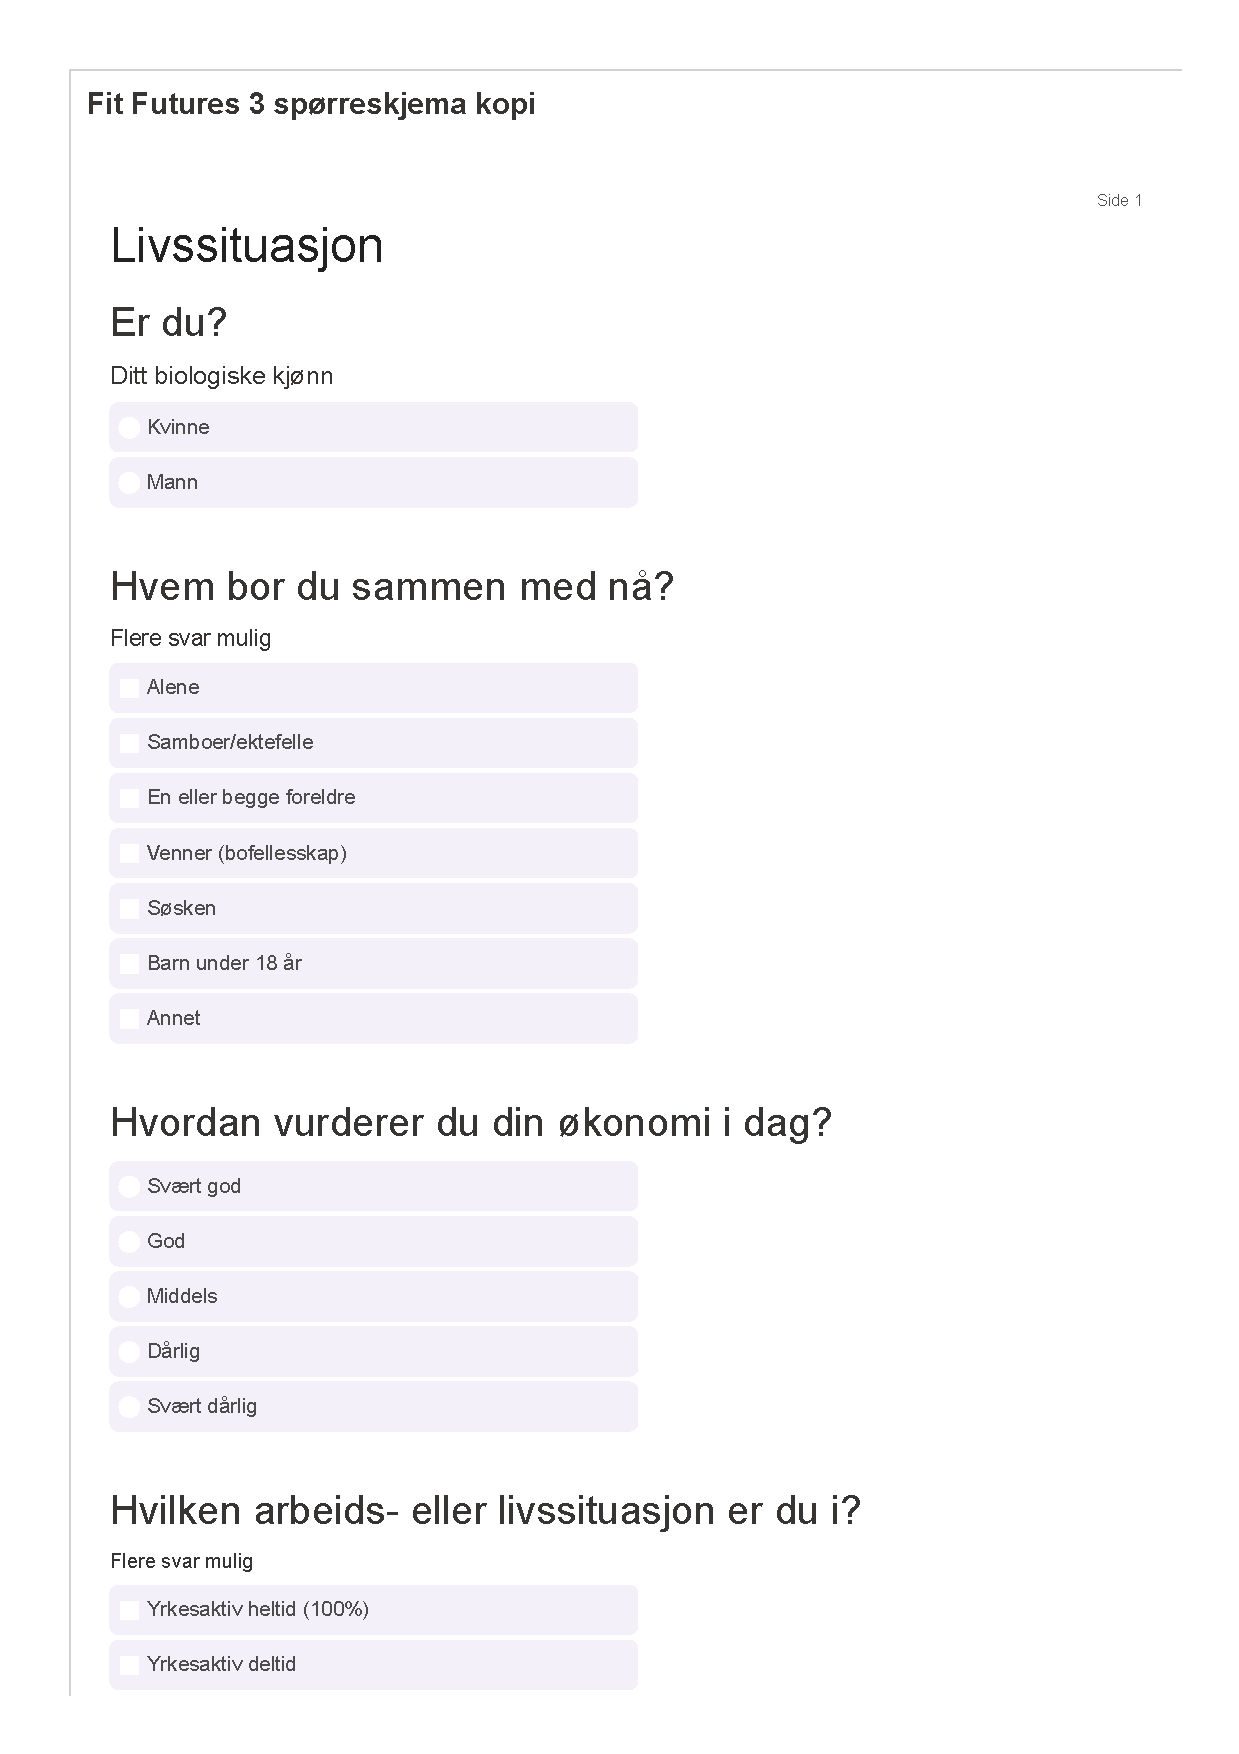
\includepdf[pages=1-32, nup=2x2, scale = 0.95, offset=30 -10]{Annex/FF3NOR_final_version.pdf}

%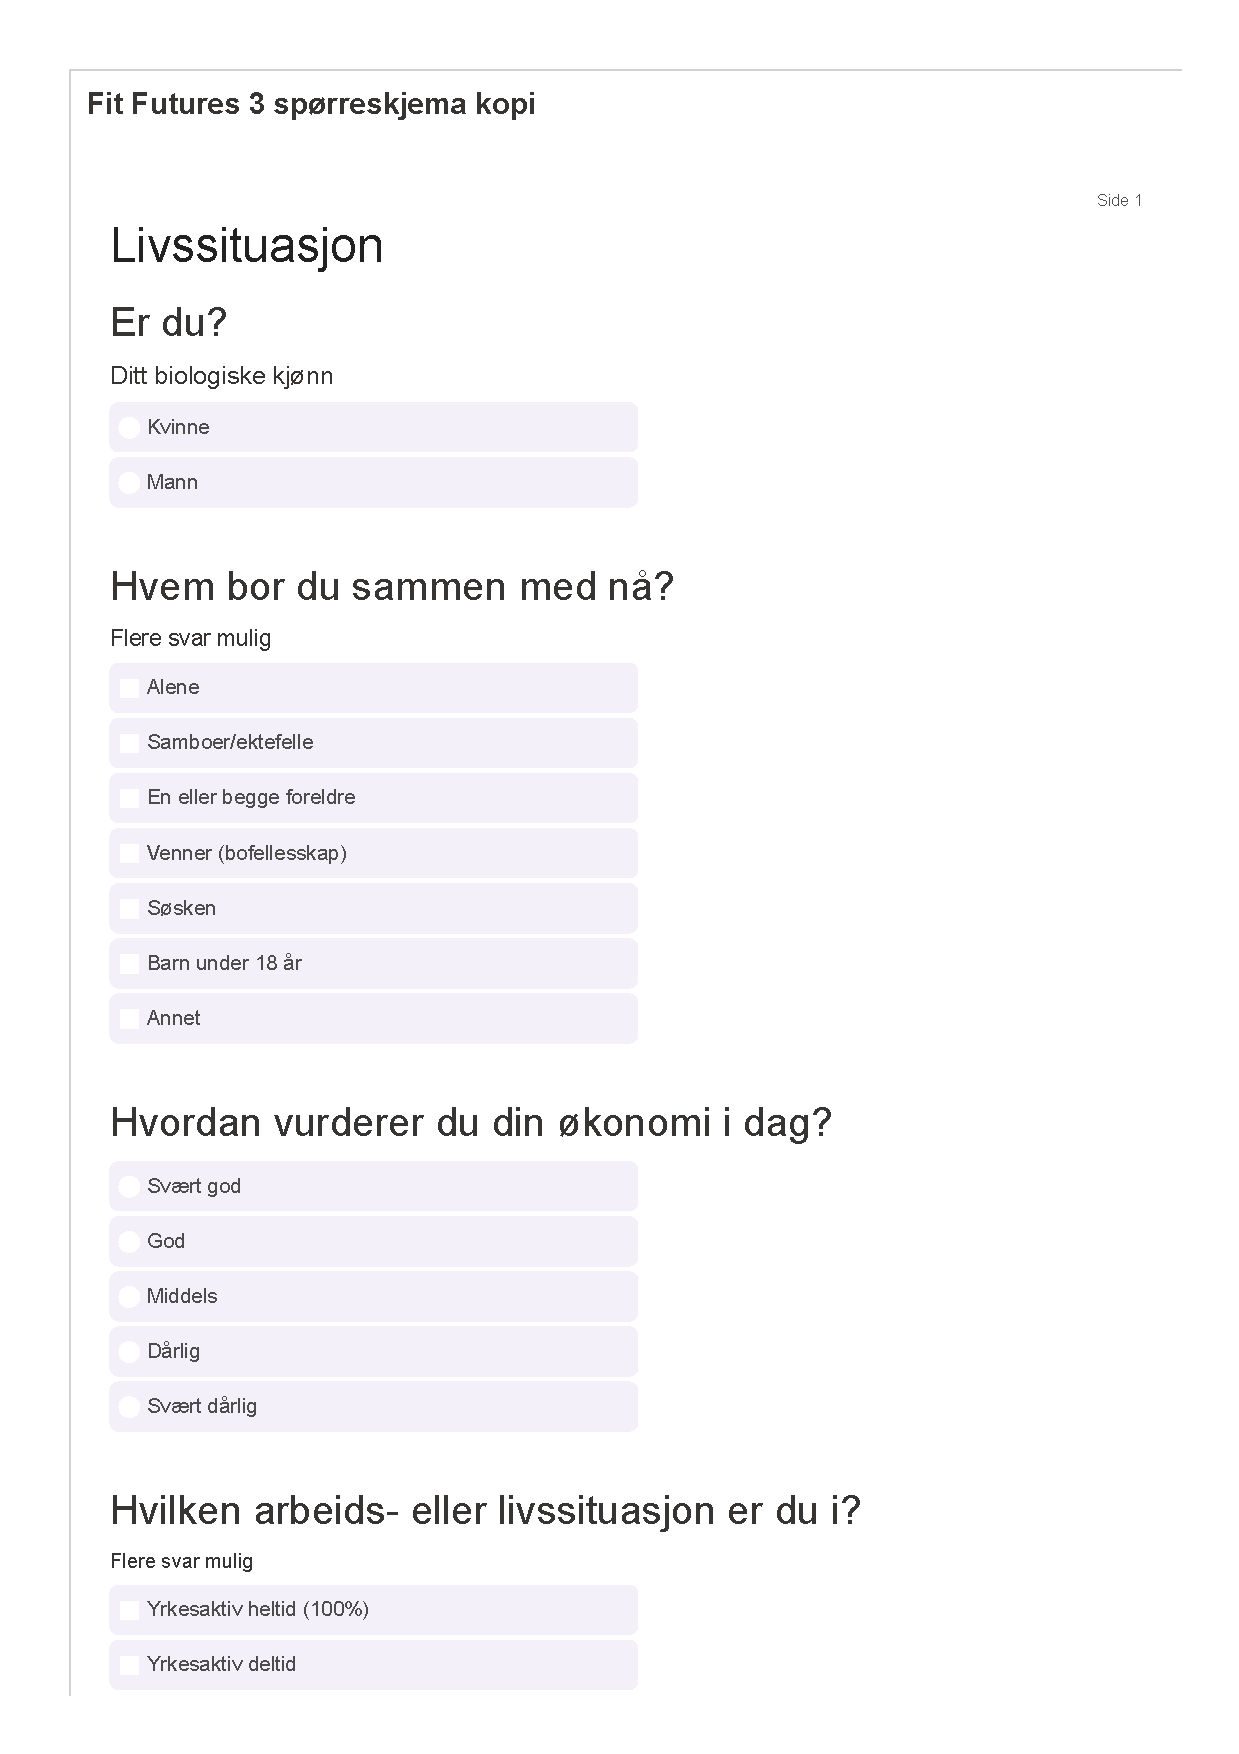
\includepdf[pages=1-32, nup=2x2, scale = 0.95, offset=0 190]{Annex/FF3NOR_final_version.pdf}

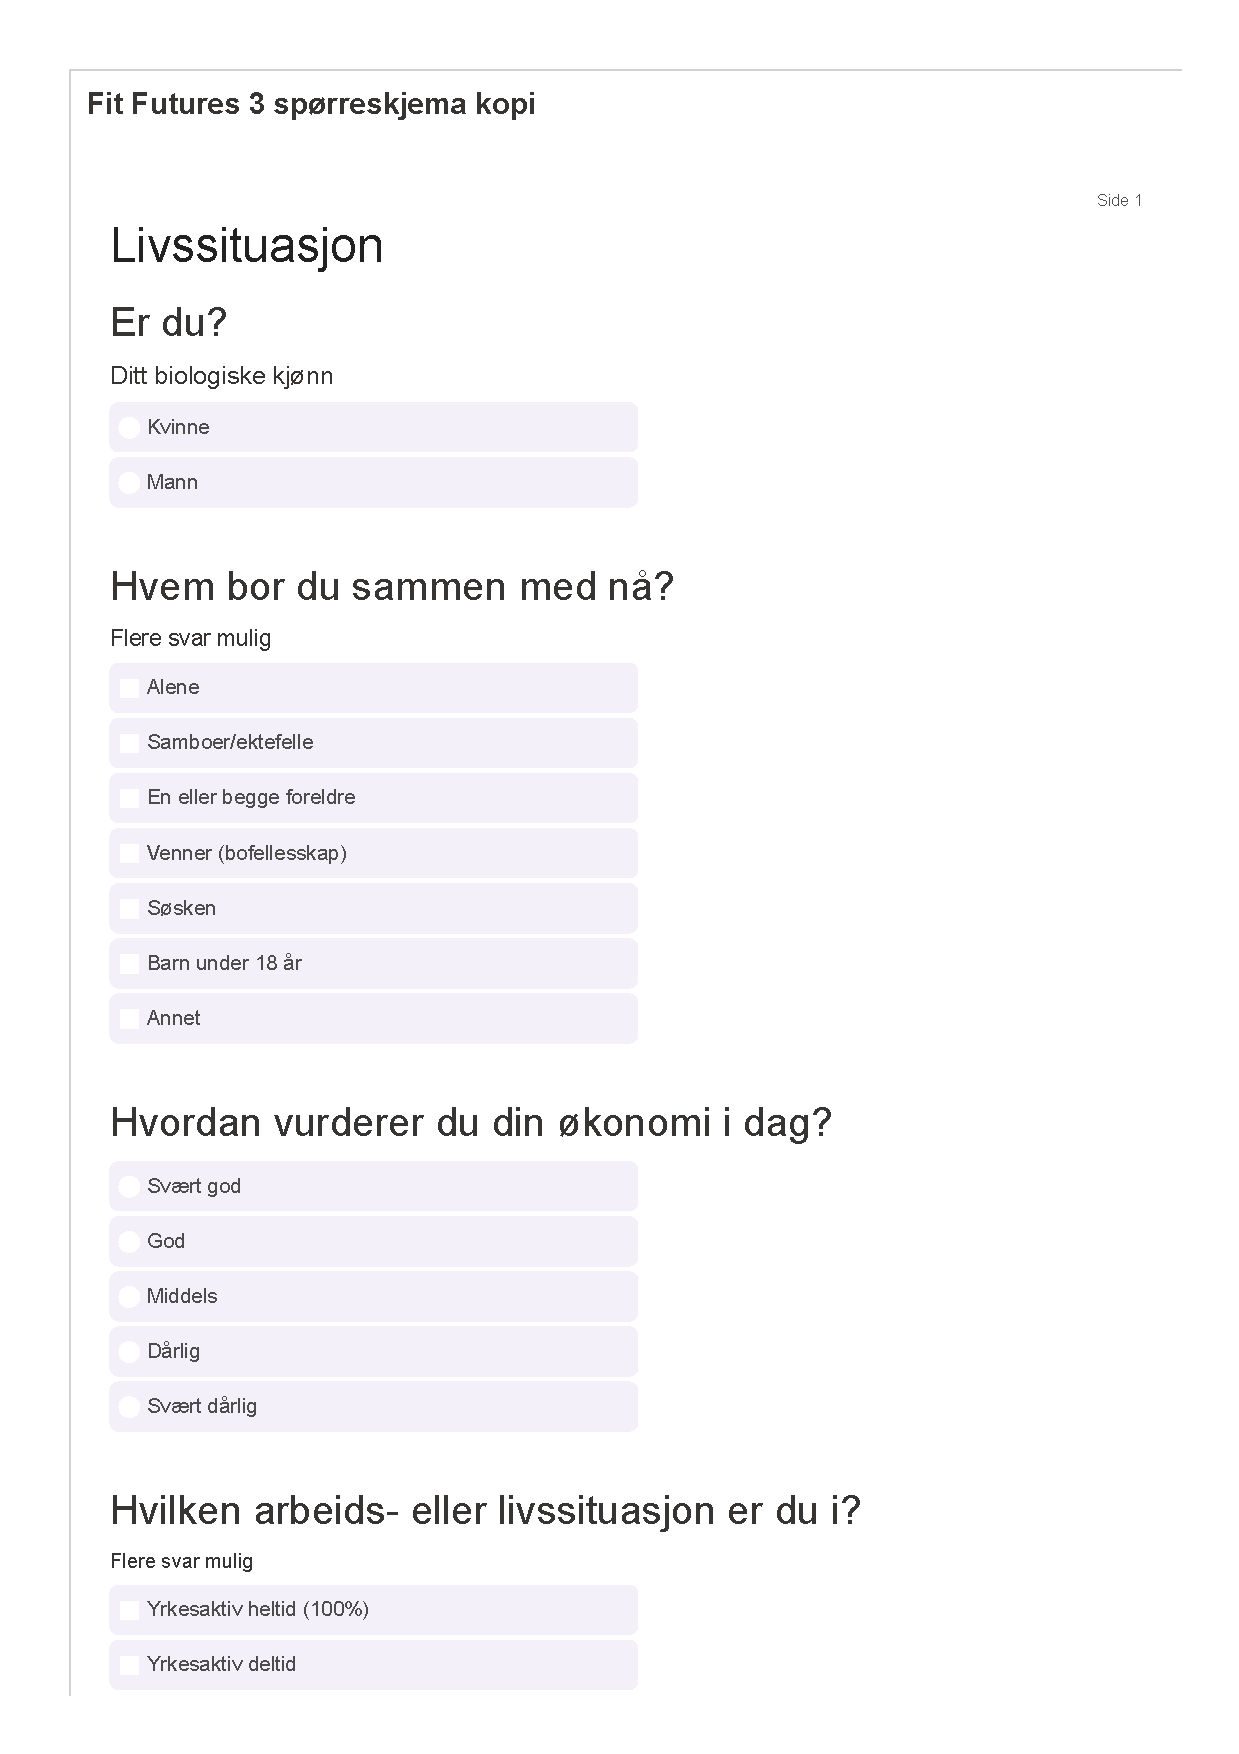
\includepdf[pages=1-32, width=\textwidth]{Annex/FF3NOR_final_version.pdf}